\documentclass{article}

\usepackage{hyperref}
\usepackage{graphicx}
\usepackage{amsmath}



\hypersetup{
    colorlinks = true,
    linkcolor = blue,
    anchorcolor = blue
}

\graphicspath{{img/}}





\title{Heat Dissipation}

\author{Davide Dal Bianco \\ 2598719}

\begin{document}

\maketitle

\section{Introduction} \label{sec:introduction}
In this report we will introduce a possible parallelization of a program that simulate the heat dissipation on a cylindrical surface. In order to simulate the dissipation, the time domain splitted in discrete points and the procedure iterates until it converges or the maximum number of iterations is reached. The program will be implemented in Cray Chapel, a modern programming language that allows to develop parallel programs using a global view programming approach, that is, the programmer solves the whole problem like a sequential program. In fact, we will provide a sequential program, a parallel single machine one and distributed one with minimal changes in the code. However, we will show that the compiler has many limitations and the overall speedup is really poor.

\section{Algorithm} \label{sec:algorithm}
The algorithm is pretty similar to Successive Over Relaxation, except that the conceptually the leftmost and the rightmost columns are adjacent. On the other hand, the top and the bottom rows have fixed values. Also the way to compute the new value of each cell is different, since it depend on a specific conductivity index of the cell and the weighted average of all 8 neighbours. \\
If the matrix is distributed among the nodes using the block distribution, the communication is $\mathcal{O}((M~+~N)~/~\sqrt{P})$ while the computation is $\mathcal{O}((M~\times~N)~/~P)$. It follows that the computation/communication ratio is good only when the problem size is much higher than the number of processes. When such condition is satisfied, the parallel algorithm is able to reach a nearly perfect linear speedup. \\
The row distribution might perform slightly better, since it does not require communication for copying the right-left columns and each process have to communicate with maximum two other processes.

\section{Sequential program}
Chapel's domain are a convenient high level abstraction for working with complex data structure. In order to compute each cell, we can use domain to execute the operation at higher level. The following domain has been defined:
\begin{itemize}
    \item \texttt{BigD}, which represents all the cell and the ghost cells.
    \item \texttt{D}, which represents all the cell to be computed.
    \item \texttt{Halo}, which represents the top-left cell and its halo.
\end{itemize}
Note that \texttt{Halo.translate(i, j)} is the domain that represents the $(i,j)$ cell and its halo. We also created the array \texttt{weights} over \texttt{Halo} where the inner cell is 0 and the other cells contain the weights for the neighbours. \\
Before starting to compute the iterations, the top-bottom ghost cells are copied (they have fixed values). Then each iteration repeats the following steps:
\begin{itemize}
    \item The left-right ghost cells are copied.
    \item Each cell $(i,j)$ is computed using the matrix restricted to \texttt{Halo.translate(i, j)}, \texttt{weights} and the conductivity index. The result is saved in a temporary matrix.
    \item The maximum difference between the old and the new value of each cell is calculated.
    \item The new values are copied in the matrix.
\end{itemize}
Using the domain \texttt{Halo}, the algorithm can be implemented very easily. However, operations like \texttt{forall} and \texttt{reduce} are not allowed because they introduce parallelism, hence the reduction must be implemented by means of a \texttt{for} iteration on the data structure.

\section{Parallel program}
In section \nameref{sec:introduction} we said the the parallel program has minimal changes compared with the sequential one. In fact, when working with complex data structures such as arrays or matrices, Chapel can execute the operations in parallel using a thread pool. The parallelization is transparent from the programmer's perspective, but he must be aware of it because race conditions might invalid the correctness of the program. \\
The resulting parallel program is identical to the sequential one, except that operations on data structures are done using \texttt{forall} loops and the \texttt{reduce} parallel operator.

\section{Distributed program}
Once again, in order to distribute the program, only minimal changes to program are required. In particular, we have to instruct the compiler that the data must be distributed and this is done using a particular syntax when definining the arrays. Chapel already provide the most popular partitioning scheme and the programmer can also implement an arbitrary one, though this is not needed in this case. As described in section \nameref{sec:algorithm}, the block distribution provided by Chapel is a good partitioning scheme. Therefore, the only change in the program is on the \texttt{BigD} domain declaration, which now is also \texttt{dmapped Block(...)}.

\section{Performance measurement}
In order to measure the performance gain, the running times of the program have been measured for the following problem sizes:
\begin{itemize}
    \item Size 1: M = 1000, N = 1000, E = 0.1, I = 100
    \item Size 2: M = 2000, N = 2000, E = 0.05, I = 200
    \item Size 3: M = 5000, N = 5000, E = 0.2, I = 500
\end{itemize}
Each execution has been repeated four times and the average time has been chosen as the most representative one, in order to provide a steadier measurement. For the multi-locale version, the program has been tested with 1, 2, 4, 8 and 16 locales.
\begin{figure}
\centering
\frame{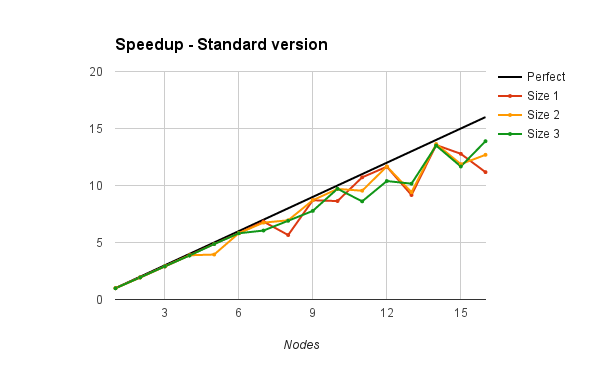
\includegraphics[width=0.8\textwidth]{speedup_standard.png}}
\caption{Speedup - Standard version}
\label{fig:speedupstandard}
\end{figure}
The chart in \autoref{fig:speedupstandard} shows that the speedup is really bad. As we said in section \nameref{sec:algorithm}, the speedup should be almost perfect and this is not the case. The reason must be found in the compiler, which is not able to produce optimized code starting from a Global View program. There are also other problems when using high level operations on arrays, therefore the program must be modified in order to help the compiler to produce better code. We will provide some optimization in section \nameref{sec:improvements}.

\section{Improvements} \label{sec:improvements}

\begin{table}
\centering
\begin{tabular}{|l|c|c|c|}
\hline
Phase & Size 1 & Size 2 & Size 3 \\
\hline
Left-Right columns copy & 0.56 (0.09\%) & 0.32 (0.03\%) & 0.39s (0.03\%) \\
\hline
Update & 2.52 (0.39\%) & 0.48 (0.06\%) & 0.41s (0.03\%) \\
\hline
Computing delta & 469.15 (73.36\%) & 501.71 (59.26\%) & 601.32s (47.88\%) \\
\hline
Matrix copy & 144.65 (22.62\%) & 149.36 (17.64\%) & 177.17s (14.11\%) \\
\hline
\end{tabular}
\caption{Execution time per phase} \label{tab:timeperphasecomparison}
\end{table}

In order to improve the program, we need more accurate metrics. In particular, we should try to improve specific phases of the program, merge different phases or delete needlese phases. We will describe the successfull and unsuccessfull attemps to improve the program in the next paragraphs.

\subsection{High level operations}
One of the main cause of the bad performance are the high level operations, that is, aritmetic operations or assignments on complex data structures (arrays). We noticed that, when iterating on the data using a \texttt{for} or better a \texttt{forall} loop and executing the operation on each element, the time required is much less. This is really weid behaviour of the compiler, since the higher level instruction could be just syntactic sugar. It is likely that the compiler fails some assumption on the domain and/or on the presence of side effects, but the measured slow down is really unbelievable. Therefore, after removing all the operations on arrays, the program had a considerable performance gain.

\subsection{Grouping operations}
The sequential program reads the entire matrix three times per iteration: first to update each cell, then to compute the maximum delta and finally to copy the temporary matrix into the standard one. While the first scan is not compatible with the third one, the first one and the second one can be grouped as well as the second one and the third one. This allow to iterate over the matrix only twice, saving a noticeable amount of time. We chose to group the last two iteration, that is, the calculation of the delta and che copy of the matrix. \\
Note that this improvement is not applicable to the parallel and distributed program since they calculate the delta using the builtin parallel \texttt{reduce} function, which is much faster.

\subsection{Avoiding matrix copy}
In \autoref{tab:timeperphasecomparison} we showed the duration of each phase of the program. Using the first two improvements, the program had a pretty big performance gain. However there is still needless work performed during the iteration. In fact, at the end of iteration the temporary matrix is copied in the regular one and this waste a lot of time. We can easily avoid the need of the copy by alternately the regular matrix and the temp matrix. In other words, given two matrix $M1$ and $M2$, in even iterations $M1$ works as regular matrix and $M2$ as temporary matrix while in odd iterations $M2$ works as regular matrix and $M1$ as temporary matrix. \\
More attention must be paid at the end of the program: the result will be in one of the two matrix according to the number of iteration.

\subsection{Avoiding needless computation}
While inspecting the conductivity pattern we noticed that many cell have value 65535, that is, the conductivity index is null. When there is no conductivity, the value of the cell remains constant over the time domain, therefore after updating the cell the value will be the same. We can exploit the conductivity index to compute a cell only when needed, avoiding useless computation, memory access and, for the multi locale version, communication.

\subsection{Avoiding delta calculation}
The convergence criterion states that, when for each cell the difference between the old value and the new computed one is below a given threshold, the algorithm terminates. In order to that, in each iteration the maximum difference for each cell is calculated and it is compared with the threshold. Though it is correct, this is not the optimal solution since it compute a lot of unnecessary information. In fact, we don't really need to know if the maximum value is below the threshold, but what we need is to know if there is at least one difference above the threshold. Introducing this little change, we don't need to explore the entire matrix but only on part of it. During the first iterations it is likely that most cells have a difference above the threshold, hence only a minimal part of the matrix must be examined.

\subsection{Stencil distribution}
In the multi locale version, we distribute the matrix among locales using the \texttt{Block} distribution. Though this approach is correct, every time a locale use an external cell it must perform a remote read. During a single iteration a locale access the same external cell about three times, therefore the locale performs three different read operations though the value is constant. \\
Chapel provide a particular distribution, namely \texttt{Stencil} distribution, which is designed for stencil operations. It is a particular block distribution, where the adjacent cells are stored in a read-only cache. This allows to read the “remote” cells in the local memory and the cache can be updated manually using the method \texttt{updateFluff}.

\subsection{Row partitioning}
In the section \nameref{sec:algorithm} we already argued that the row partitioning might perform slightly better, since it does not require communication when copying the right-left boundaries. The implementation is really easy, since the Block (or Stencil) distribution constructor has the parameter \texttt{targetLocales} which allows to set how data must be mapped to locales. In this particular case, targetLocales should be a matrix which width is 1.

\subsection{Keyword local}
The Chapel compiler is not yet able to produce well optimized code. Sometime it fails some easy assumpions about data locality and this introduce a big communication overhead. However, the programmer can tell the compiler that some code perform only local memory access using the keywork \texttt{local}. In particular, the keyword can be used in two parts of the program:
\begin{itemize}
    \item When copying the right-left columns, since we are now using a row distribution.
    \item When updating each cell, since we are using a Stencil distribution and the cache is updated manually.
\end{itemize}
After this change, the program had an incredible performance boost due to the less communication involved.

\end{document}